\documentclass[a4paper,11pt]{article}
\usepackage[utf8]{inputenc}
\usepackage{graphicx}
\usepackage[english]{babel}
\usepackage[vmargin=3.5cm, top=2cm]{geometry}
\usepackage[linktocpage=true]{hyperref}
\usepackage{enumitem}
\usepackage{longtable}
\usepackage{pdfpages}
\usepackage{float}
\usepackage{hyperref}
\usepackage[section]{placeins}
\hypersetup{
   colorlinks,
   citecolor=black,
   filecolor=black,
   linkcolor=black,
   urlcolor=black
}

\begin{document}

\begin{titlepage}

\centering \parindent=0pt
\newcommand{\HRule}{\rule{\textwidth}{1mm}}
\vspace*{\stretch{1}} \HRule\\[1cm]\Huge\bfseries
Graphics Programming Report\\[0.7cm]
\HRule\\[4cm]  
\large by 
\\Alexander Kirk
\\ and Mikkel Stolborg
\vspace*{\stretch{2}} \normalsize %
\begin{flushleft}
IT University of Copenhagen \\
GRPRP, S2015\\
Dan Lessin\\
\today \end{flushleft}
\end{titlepage}

\tableofcontents
\pagebreak
\section{Introduction}
Solar system simulation choice.
For this project we decided to create a simulation of the solar system with the planets acting on each other using gravitational forces. The idea was to have the sun act as a point light and the planets move only with a set starting velocity, having the forces move them accordingly and the lightning of the sun ensure the planets are lit accordingly.

\section{Week structure}
In the following sections we will go through the work done each week and who did the work on each of the individual task.
\subsection{Week one - Initialization and project development}
The first week were spent creating the basics of our project. The foundation of the final scene and the objects for the calculations. 
We set up a git structure to hold the project.
For the graphical side of the project there was created a basic scene with a sphere object to symbolise the final planets of our project. The methods for loading the sphere and lighting the basic light of the scene were implemented.
As the counterpart we created the basics classes for handling the physics calculations. They would calculate the the gravitational pull of each object against each other. The objects would be moved according to the acceleration imposed on them from the gravitational pull. 
The general structure were bound together through a over class which kept the graphical and the physical structure in separate classes linked through a common position value kept in a simulation object, see figure \ref{GraphicsObjects}.
\begin{figure}[h]
\centering
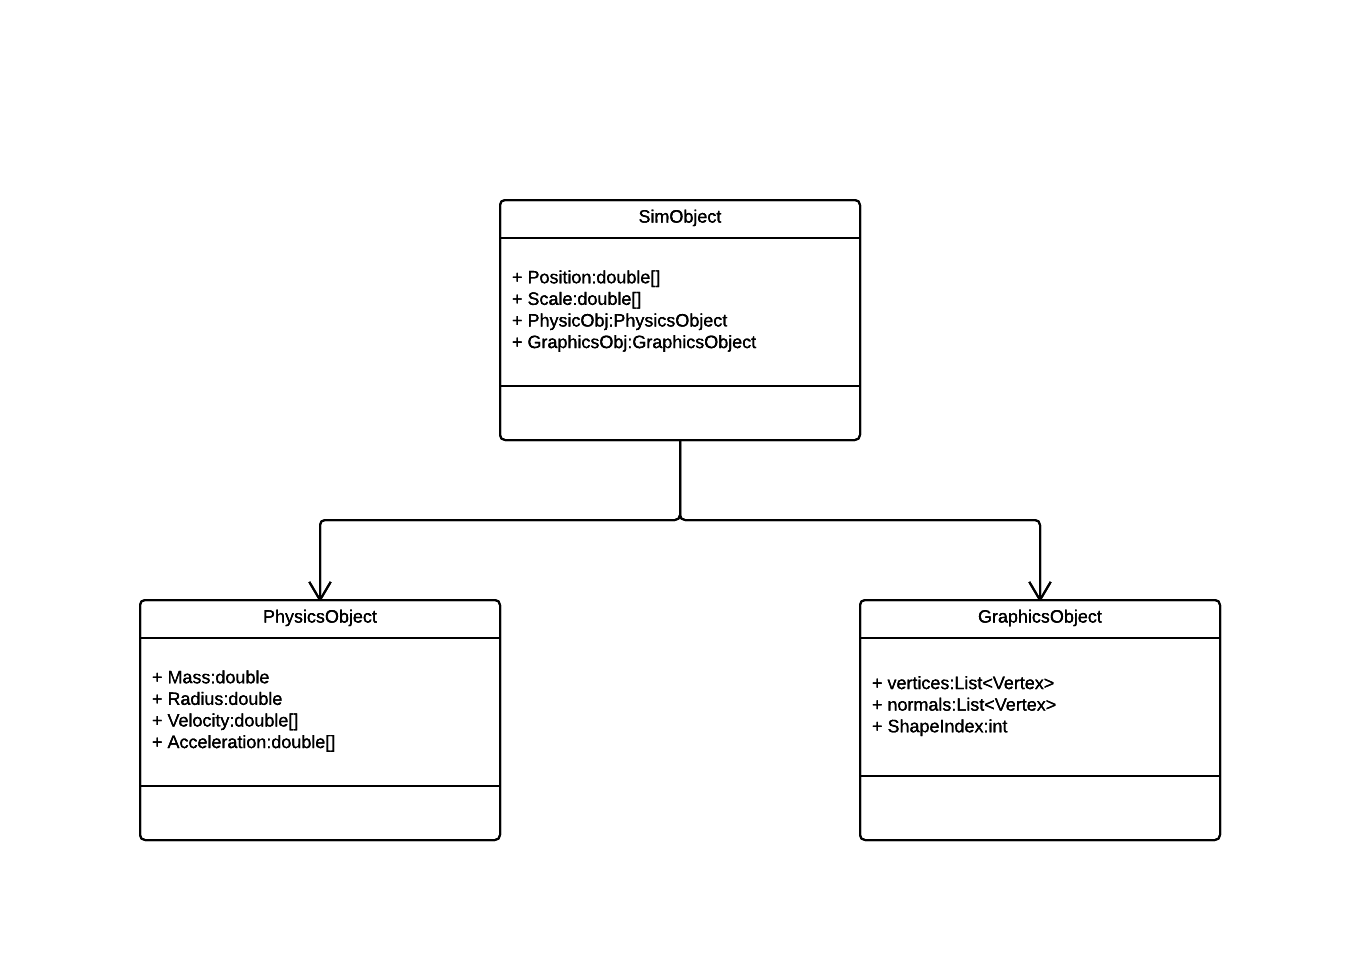
\includegraphics[scale=0.7]{GraphicsProjectObjects.png}
\label{GraphicsObjects}
\caption{Structure of the simulation objects and their physics and graphic objects}
\end{figure}
\subsection{Week two - Integration and transformation}
This week we integrated the different parts of the project for a unified physics and graphical simulation. There was some problems with graphical and physical integration, were the positions were not updated. 
Even after the integration were completed. There were some problems with moving the camera so that we could follow the moving planets. 
The physics were updated to produce transformation matrices which should move the objects around in the simulation. These change the current position of the graphical object. They needed to be moved through translation of their vertices which required a translation matrix.
\subsection{Week three}
Implementation of comet initialisation
Shading algorithm.

\subsection{Week Four}
Polishing of project and preparation for presentation
\section{Results}
Overlook of current implementation, pictures and explanation
\section{Conclusion}
Finalization of goal and end result

physics are working 
\end{document}